\newpage
\chapter{Опис досліджуваних зразків}
\section{Наноструктуровані $pHEMA-TiO_2$ гібридні матеріали}
The exceptional electronic properties of these hybrids are
related to those of TiO2 colloids discovered a long time ago,11 in
which the electron–hole separation efficiency under UV illumi-
nation was reported below 16%, resulting in their visible dark-
ening due to the trapped electrons. The absorption of a photon
results in the electron transition from the valence band (VB)
formed by O2À 2p-orbitals to the conduction band (CB) due to
Ti4+ 3d-orbitals.12 The eÀ–h+ recombination can be prohibited in
the alcohol solutions, which rapidly scavenge the photogenerated
VB holes. This is consistent with a high electron loading capacity
of 112 mM MÀ1 (Ti) observed in new porous TiO2 materials.13
Dissociation of excitons at the organic–inorganic nano-interface
can enhance the photocarrier generation. The related mechanism
is a basis for relevant charge-separation devices and intimately
mixed at nanoscale biphasic materials deserve now much
attention.

The TiO2 gels are not fundamentally different from colloids,
since they are colloidal in nature and formed by nanoparticles.
As our studies have shown16,17 titania alcogels offer even higher
charge separation efficiency of \~20–25\%. In our previous
papers,18,19 we have developed new photochromic pHEMA/
TiO2-gel based hybrids (pHEMA 1/4 poly(2-hydroxyethyl meth-
acrylate)) with a high charge separation efficiency of 12The TiO2 gels are not fundamentally different from colloids,
since they are colloidal in nature and formed by nanoparticles.
As our studies have shown16,17 titania alcogels offer even higher
charge separation efficiency of \~20–25\%. In our previous
papers,18,19 we have developed new photochromic pHEMA/
TiO2-gel based hybrids (pHEMA 1/4 poly(2-hydroxyethyl meth-
acrylate)) with a high charge separation efficiency of 12\% and
electron loading capacity of 14\%. Furthermore, we have
observed that the electron transfer depends on the material
microstructure, which can be affected by the materials chemistry
and processing. Tuning a delay between the inorganic poly-
condensation (gelation) and organic polymerization stages of the
system allows optimisation of the photochromic responses of the
resulting nanocomposites.19 As these studies show, the building
inorganic nanounits have a crucial importance for the material
photonic sensitivity. In particular, hybrids formed of smallest
Ti16O16(OEt)24(OEMA)8 nanobuilding block (OEMA is the
deprotonated form of HEMA) covalently linked to the organic
polymer pHEMA were developed:20–22 these structurally\% and
electron loading capacity of 14\%. Furthermore, we have
observed that the electron transfer depends on the material
microstructure, which can be affected by the materials chemistry
and processing. Tuning a delay between the inorganic poly-
condensation (gelation) and organic polymerization stages of the
system allows optimisation of the photochromic responses of the
resulting nanocomposites.19 As these studies show, the building
inorganic nanounits have a crucial importance for the material
photonic sensitivity. In particular, hybrids formed of smallest
Ti16O16(OEt)24(OEMA)8 nanobuilding block (OEMA is the
deprotonated form of HEMA) covalently linked to the organic
polymer pHEMA were developed:20–22 these structurally
well-defined Ti16-based nanocomposites differ essentially from
the other hybrids by nature of the internal interface and
confinement of the photoactive sites and show a relatively low
photonic sensitivity.

An important task in order to further increase the material
photonic sensitivity is to properly design the nanoscale bulk
interface between TiO2 and polymer that enables the charge
injection into two different material components: VB-hole
escapes into the organic one and CB-electron remains onto the
inorganic one as Ti3+ polaron-like centre. In this sense, the
nanoscale unit size has to be optimized and macroscopic quantity
of the identical nanounits has to be assembled into the high-
optical quality bulk material.

In the present communication we propose an original solution
to the above problem by the size-selective fabrication of oxo-
TiO2 nanoparticles, their surface exchange and covalent binding
into a polymer network, which allows the material morphology
control.


\subsection{Hybrid preparation}
A polymerisation of the HEMA–
TiO2 precursor was realised in the present work thermally with
the addition of an AIBN initiator to the nanoparticulate
precursor. Non-colored transparent hybrids were obtained after
24 h of heating at a temperature of 75 0 C. Mabilleau et al.34 have
recently proposed to monitor the monomer polymerization by
Raman spectroscopy, observing characteristic vibrational peaks
of C]C at 1407 and 1641 cmÀ1, associated with C]CH2
stretching and C]C aliphatic stretching vibrations, respectively.
The Raman spectra of our several obtained hybrids are shown in
Fig. 3. They evidence a complete polymerization of the pure
HEMA (b) and HEMA–TiO2 precursor with Ti concentration of
0.15 M (c). Indeed, the intensity of the two C]C bands vanishes;
at the same time, the intensity of the C–C band at 1455 cmÀ1
associated with the deformation of the C–H group increases
indicating the elongation of the polymeric chain. On the other
hand, some intensity of the C]C peaks remains when the
nanoparticle loading increases (Fig. 3d). Higher temperature
treatment is known to provide diffusion possibilities and allows
better steric adjustment for the efficient organic polymerisation
of HEMA moieties. We have observed that both longer (75 0C/
48 h) and higher temperature (90 0C/24 h) treatments decrease
the non-polymerised organic component by up to 30\%
(temperatures above 110  0C were skipped in the present study,
since they produce non-desirable yellowish coloration of
samples). No systematic quantitative estimations of the extent of
polymerisation were carried out because no safe procedure is
available for peak normalisation between different samples.
However, residual HEMA monomers were always observed in
most concentrated hybrid samples ($C_{Ti} >= 1.5$M) indicating that
the corresponding organic polymerisation is extended but
incomplete.

The nanoscale morphology of the prepared hybrid materials
(size, shape and distribution of TiO2 particles in pHEMA poly-
mer matrix) was characterised by JEOL2011 high resolution
transmission electron microscopy (HRTEM) operated at
200 keV with an emission type LaB6 (field emission). Also,
a Gatan Imaging Filter 2000 system connected to the TEM
offered us access to element maps, by energy filtered transmission
electron microscopy (EFTEM). The resolution of the energy
filter is 1 eV and the dimensional resolution is 1 nm. The corre-
sponding images of the polymer (a) and hybrid (b and c) with
titanium molar concentrations of 3.0 M are shown in Fig. 4. A
comparison between HRTEM images (a) and (b) evidences
a strong modification of the material morphology at nanoscale:
while disordered polymer chains are observed in pure pHEMA,
the polymer structure is superposed with that of the inorganic
component in the hybrid. The unit size of the bright Ti domains
(c) can be estimated as \~4 nm, which is in agreement with the
core size of the colloidal precursor nanoparticles (if the OEMA
ligand length is subtracted from their hydrodynamic size of
5.0 nm). The nanoparticles are not aggregated with the mean
interparticle distance close to the particle size. It seems, however,
that the polymer chains are more organized in the hybrid than in
the pure pHEMA, forming locally quasi-ordered domains with
the period of 0.6–0.7 nm that can terminate/originate on/from
nanoparticles. This may be a reason for not complete polymer-
isation of the hybrids.

\begin{figure}
\centering
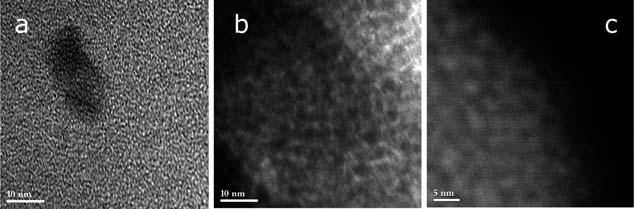
\includegraphics[width=12cm]{em} 
\caption{HRTEM (a and b) and EFTEM (c) images of pHEMA (a) and
pHEMA–oxo-TiO2 hybrid (b and c) with titanium molar concentrations
of 3.0 M.	}
\end{figure}

%\subsection{Photonic sensitivity}
%
%The interfacial charge-transfer in TiO2 gels,9,16 crystalline tita-
%nium alkoxide compounds13 and organic–inorganic hybrids18,19
%enables domains with modified absorption, refraction, conduc-
%tive and magnetic properties. Our fabricated hybrids differ from
%these previous materials by much lower polydispersity of the
%structural nanounit, which has an impact on the photochromic
%behaviour. The broadband UV–visible–IR absorption (dark
%continuum) has been earlier assigned to shallow (De z 0.5 eV)
%polaronic Ti3+ centres. The charge storage process is associated
%with the rapid VB-hole exit and scavenging into the organic
%component followed by the localisation of a heavier CB-electron
%onto Ti4+ of the inorganic component. The process efficiency
%depends on the nature and extent of the hybrid interface which
%can be tailored through the materials chemistry and processing.
%
%We have measured the photonic sensitivity of the prepared
%hybrids in pump-probe experiments, with nanosecond UV pump
%laser irradiation (MOPO by Spectra Physics: 7 ns, 355 nm). The
%pHEMA–TiO2 sample was shaped into a thin slab of 150 mm
%thickness and irradiated at normal incidence. The laser pulse-to-
%pulse energy was continuously monitored by J4-09 black coating
%sensor (Coherent). The sample absorbance was probed in situ by
%the collinear beam from a stabilized cw-laser diode module at l 1⁄4
%640 nm, which spectrally fits the maximum of the Ti3+ visible
%continuum. To avoid signal contamination by the pump laser,
%each measurement point was accomplished during the time
%interval between two successive UV-laser pulses. The trapped
%electron concentration was calculated by using absorption cross-
%sections of both Ti4+ (355 nm) and Ti3+ (640 nm) centres, corre-
%sponding to 4.3 Â 10À20 cm2 and 1.3 Â 10À18 cm2 previously
%measured by simultaneous absorption and electronic para-
%magnetic resonance experiments.35 The data collection in real
%time was assured by LabView software.
%
%The series presented in Fig. 5 was carried out with UV-laser
%fluence of 30 mJ cmÀ2. However, similar data were obtained with 3
%times lower laser fluence of 10 mJ cmÀ2, which shows a negligible
%contribution of thermal and spontaneous relaxation processes in
%agreement with Kuznetsov et al.19 In agreement with the proposed
%model of the photoinduced processes in TiO2 gels and hybrids,16,19
%our present results evidence an efficient photoinduced charge
%separation in the prepared samples g 1⁄4 dNTi /dNph 1⁄4 50% (Fig. 5a)
%as well as high charge storage capacity of Q 1⁄4 NTi /NTi 1⁄4 12%
%
%(Fig. 5b). The measured efficiency is to our knowledge the highest
%one reported up-to-date: it is more than a factor 4 higher than best
%previously reported values in the hybrid systems19 and 2 times
%higher compared to that in TiO2 alcogels.17 The concentrated
%hybrids produced from our nanoparticulate precursor conserve the
%high photonic sensitivity. Our measurements of the hybrid with
%even higher nanoparticle loading (CTi 1⁄4 3.0 M) do not lead to any
%lowering of the (g,Q) values. According to Kuznetsov et al.,19 the
%quantum efficiency of the photoinduced charge separation depends
%on the light VB hole lifetime in the vicinity of the heavier CB elec-
%tron before it escapes onto the organic component. The consider-
%able improvement of g supports our previous conclusion about the
%key role of an organic–inorganic interface: both measured (g,Q)
%values can than be considered as intrinsically related to the interface
%morphology (nature of components, particles size and poly-
%dispersity)

%\begin{figure}
%\centering
%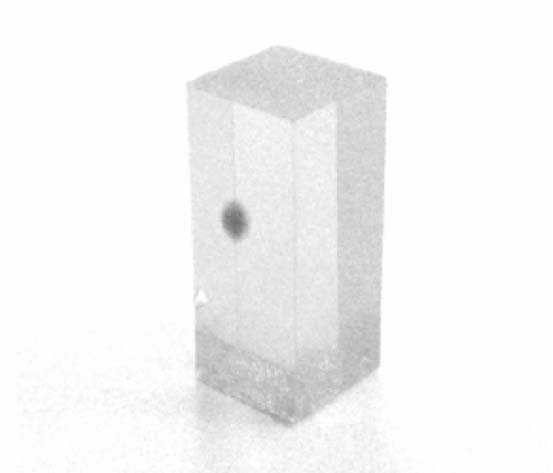
\includegraphics[width=5.5cm]{fig1} 
%\caption{Гібридний органо-неорганічний матеріал, що містить мережу з діоксиду титану після впливу ультрафіолетового випромінювання ($\lambda=355$ нм): опромінена точка стає чорною. Розміри паралелепіпеду $4~\times~4~\times~10~ mm^3$.}
%\end{figure}
